\chapter{Mediciones y configuración experimental \label{chap:ConfiguracionExperimental}}
%%%%%%%%%%%%%%%%%%%%%%%%%%%%%%%%%%%%%%%%%%%%%%%%%%%%%%%%%%%%%%%%%%
%%%%%%%%%%%%%%%%%%%%%%%%%%%%%%%%%%%%%%%%%%%%%%%%%%%%%%%%%%%%%%%%%%
\section{Configuración experimental}
\subsection{Cámara de vacío}
\noindent El detector se encontraba colocado dentro de una cámara de vacío fabricada a partir de cubo macizo de aluminio de $20\,\si{cm}$ de lado, denominado \textit{dewar}. Fue necesario que las temperaturas se encontraran por debajo de los $140\,\si{K}$ para disminuir la producción de cargas en el silicio por fluctuaciones térmicas (corrientes oscuras), como así también el fondo producido por fotones infrarrojos emitidos por las superficies interiores del \textit{Dewar}, que se encontraban a temperatura ambiente.
\begin{figure}%[h]
    \centering
    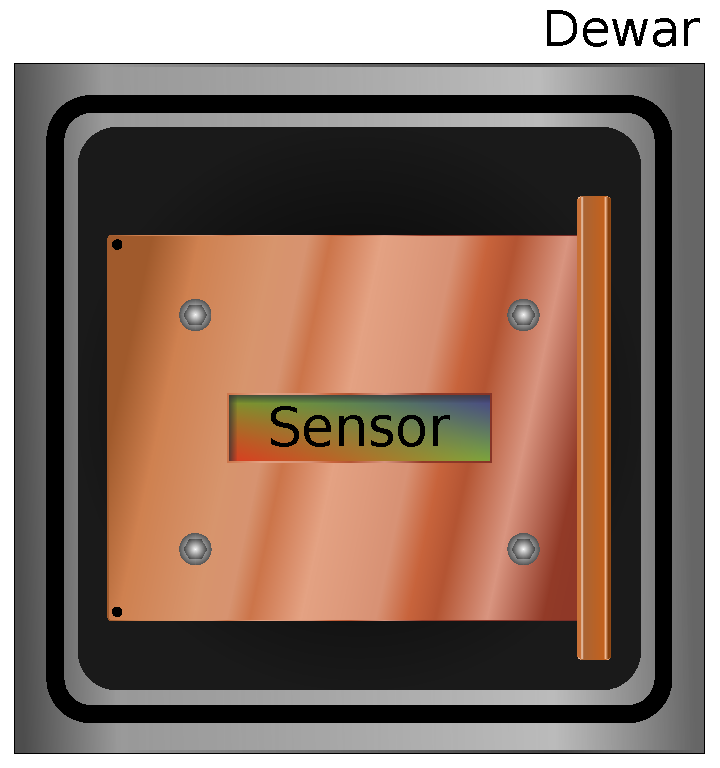
\includegraphics[scale=0.5]{Figs/Frontal_Dewar_Sensor.pdf}
    \caption{\footnotesize{Esquema frontal del Dewar y el posicionamiento del sensor. El sensor se encuentra montado detrás de una placa de cobre frontal con un abertura rectangular por donde la radiación incidente alcanza al sensor. A su vez, se cubren las esquinas laterales del sensor con dos láminas de cobre para evitar la exposición de esas regiones del sensor donde es desplazada la carga para posteriormente ser medida.}}
    \label{fig:FrontalDewarYSensor}
\end{figure}
Debido a las bajas temperaturas y para evitar la condensación de humedad dentro del recinto, se hizo vacío mediante la utilización de una bomba turbo-molecular, capaz de alcanzar una presión del orden de los $10^{-5}\,\si{mbar}$.\\
\indent También fue necesaria la utilización de un calentador para controlar la temperatura del sensor y del \textit{Dewar} por dos razones principales: Evitar que la temperatura de operación del sensor sea menor a $110\,\si{K}$, debido a que la eficiencia de la transferencia de carga entre píxeles del sensor se ve disminuida para temperaturas menores a esta; y para regular la velocidad de enfriamiento del sensor, dado que podría comprometerse su integridad estructural si esta superaba $1\,\si{K/s}$.\\
\subsection{Detector utilizado}
\noindent El detector utilizado fue un \textit{fully-depleted} CCD, del tipo \textit{bulk-iluminated}, es decir, que se expone a la radiación incidente una de sus lados y luego las cargas generadas se migran hacia el lado contrario. La zona muerta en la parte trasera del CCD estaba compuesta por tres capas: Una capa de $\sim 20\,\si{nm}$ de óxido de indio y estaño (ITO, por sus siglas en inglés: \textit{Indium Tin Oxide}), una capa de $\sim 38\,\si{nm}$ de dióxido de circonio (ZrO$_{2}$) y una última capa de $\sim 100\,\si{nm}$ de dióxido de silicio (SiO$_{2}$). El CCD estaba dividido en cuatro cuadrantes, denominados OHDU, con un amplificador en la esquina de cada cuadrante, permitiendo la lectura en simultaneo de todos ellos. Cada cuadrante consiste en $2063$ filas y $500$ columnas, y cada píxel tiene una dimensión de $15\,\si{\mu m} \times 15\,\si{\mu m}$.
%%%%%%%%%%%%%%%%%%%%%%%%%%%%%%%%%%%%%%%%%%%%%%%%%%%%%%%%%%%%%%%%%%
%%%%%%%%%%%%%%%%%%%%%%%%%%%%%%%%%%%%%%%%%%%%%%%%%%%%%%%%%%%%%%%%%%
\subsection{Fuente de \texorpdfstring{$\Am{241}$}{Am241}}
\noindent Para las mediciones estudiadas en este trabajo, se utilizó una fuente radioactiva de $\Am{241}$ electrodepositada, que emitía partículas alfa con energía de $\sim 5.6\,\si{MeV}$, una actividad de $1\,\si{\mu C}$ y un diámetro de $5\,\si{mm}$. Para obtener los rayos $X$ de fluorescencia del flúor y del aluminio, se colocó dentro del \textit{dewar} un caja de cobre enfrentada al sensor y que alberga una cinta de Teflón, material que contiene flúor, y una placa de aluminio. La fuente radioactiva se colocó debajo de esta caja de cobre, a la cual se le hizo un agujero por donde ingresaban las partículas alfa que impactarían los materiales para producir la fluorescencia, como se ve en el esquema de la figura \ref{fig:FrontalAlYF}.
\begin{figure}[h]
    \centering
    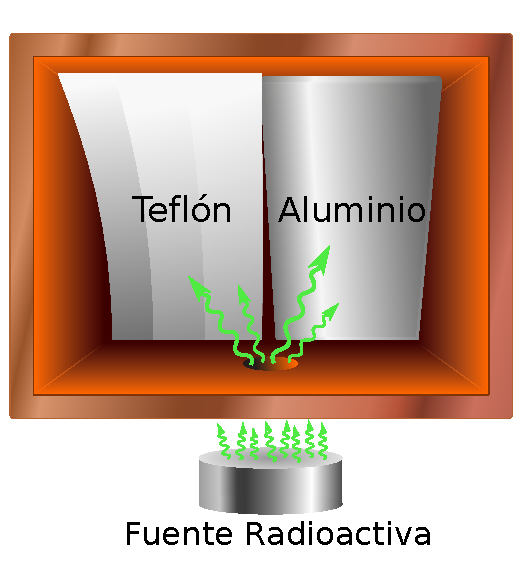
\includegraphics[scale=0.7]{Figs/CajaSensor.pdf}
    \caption{\footnotesize{Esquema frontal de la caja de cobre donde se posicionaron la cinta de teflón y la placa de aluminio. Se esquematiza el orificio por donde ingresan las partículas alfa, pero no la barrera allí colocada. El sensor se encuentra montado frente de esta, detrás de la placa de cobre del esquema de la figura \ref{fig:FrontalDewarYSensor}, de forma que los rayos de fluorescencia producidos por el aluminio y el teflón impacten sobre él.}}
    \label{fig:FrontalAlYF}
\end{figure}
Además, se colocó una pequeña barrera de cobre entre el orificio la fuente y el sensor para que las partículas alfa no llegasen directamente hacia este.

En el esquema de la figura \ref{fig:LateralDewar} puede verse un corte lateral del \textit{dewar}. Del lado derecho se encuentra la caja de cobre que contiene el material que se quiere estudiar (flúor o aluminio) y la fuente radioactiva. Del lado izquierdo puede verse la estructura que sostiene el detector y la pieza de cobre destinada a regular la temperatura del mismo.
\begin{figure}%[h]
    \centering
    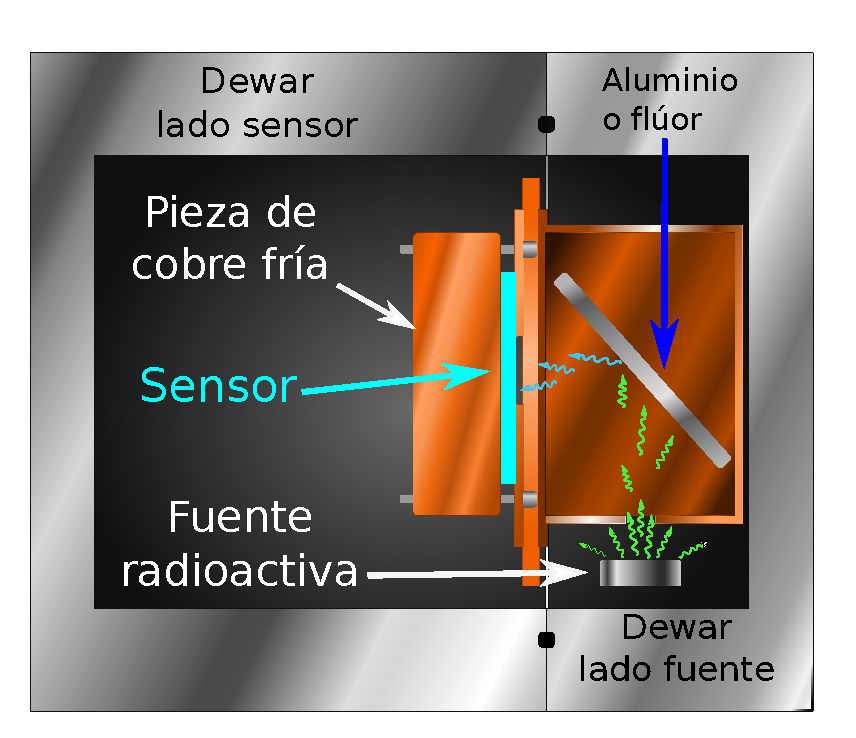
\includegraphics[scale=0.7]{Figs/LateralDewar.pdf}
    \caption{\footnotesize{Esquema lateral del \textit{Dewar}. Del lado izquierda se encuentra la placa de cobre con la abertura para el sensor (vista lateral del esquema \ref{fig:FrontalDewarYSensor}) el cual está en contacto con una pieza de cobre fría para mantenerlo en, por ejemplo, $123\,\si{K}$. Del lado derecho se encuentra la caja de cobre con la pieza de aluminio o de flúor, posicionada en ángulo y por encima del orificio por donde pasan las partículas alfa de la fuente radioactiva (vista lateral del esquema \ref{fig:FrontalAlYF}).}}
    \label{fig:LateralDewar}
\end{figure}
Por otro lado, como los fotones de la fuente radioactiva eran capaces de impactar en cualquier parte de la superficie de la caja de cobre, este podría emitir fotones de fluorescencia indeseados. Para evitar esto se recubrió el interior de la caja de cobre con cinta \textit{Kapton}, la cual está compuesta por moléculas que también pueden emitir fotones de fluorescencia, los cuales son de menor energía que los del flúor y aluminio. Esto presupone un otra fuente de fondo para las mediciones de los espectros.
%%%%%%%%%%%%%%%%%%%%%%%%%%%%%%%%%%%%%%%%%%%%%%%%%%%%%%%%%%%%%%%%%%
%%%%%%%%%%%%%%%%%%%%%%%%%%%%%%%%%%%%%%%%%%%%%%%%%%%%%%%%%%%%%%%%%%
\section{Mediciones}
\noindent Las mediciones se realizaron exponiendo la parte central del sensor a la radiación incidente y dejando los laterales donde se encuentran los amplificadores cubiertos por láminas de cobre, como se ve en el esquema de la figura \ref{fig:FrontalDewarYSensor}, para evitar su exposición. Los cuatro cuadrantes del sensor son expuestos por un muy breve período de tiempo a la radiación, para rápidamente desplazar la carga colectada en esta región a la región del sensor cubierta por las láminas y protegerla de la radiación durante el proceso de lectura. Es importante notar que el tiempo que se demora en desplazar la carga de la región expuesta a la región cubierta depende de la cantidad de columnas del sensor que se quieren medir. Si por ejemplo, quieren medirse $50$ columnas, la columna número $50$ abandonará la región expuesta en un tiempo $t$. Pero si lo que se quiere es medir $100$ columnas, entonces en este caso la columna número $100$ abandonará la región expuesta en un tiempo $\sim 2t$. Esto implica que la cantidad de eventos medidos es proporcional a la cantidad de columnas que se quieran medir.

%\noindent Debido a que la tasa de eventos de fluorescencia de aluminio y flúor producidos fue relativamente baja, las colección de eventos se realizó exponiendo el detector durante $20$ minutos antes de realizar la medición de la carga en los píxeles. 
Para la medición de la carga de los píxeles se realizaron $300$ muestreos por píxel, lo que corresponde a un tiempo de lectura de $\sim 10$ minutos por imagen. De las $500$ columnas que tiene el sensor, se utilizaron solo $50$ para las mediciones del flúor, y de las $2063$ filas se utilizaron $500$, donde las $7$ primeras son de \textit{pre-scan}, $443$ de región activa y las $50$ finales de \textit{over-scan}, con lo cual el área activa total del sensor fue de $22150$ píxeles.

Luego de la lectura, las $300$ mediciones tomadas para cada píxel fueron promediadas y los píxeles vacíos del \textit{over-scan} fueron usados para calcular y extraer la linea de base de cada fila. Este proceso es necesario para la calibración, para poder establecer el valor en ADU's correspondiente al $0$ de carga para cada una de las filas del sensor. Las regiones de \textit{pre-scan} y \textit{over-scan} son regiones del sensor que no están colectando carga junto con la región activa, pero cuando se realiza la medición de los píxeles y las cargas son desplazadas secuencialmente, estos píxeles atraviesan la región del sensor expuesta y en consecuencia tienen una probabilidad muy baja (aunque no nula) de colectar algún evento al desplazarse hacia el nodo de sensado. Esa baja probabilidad de colectar carga durante el proceso de lectura es la razón por la cual esos píxeles son utilizadas para definir la linea de base de cada fila. Al final de cada ciclo de exposición/lectura, toda la carga colectada por el CCD era removida en un rápido proceso que toma aproximadamente un segundo.

Las imágenes resultantes contienen $443 \times 50$ píxeles por cada cuadrante y la carga es medida en unidades electrónico digitales (ADU's), que posteriormente fueron convertidas en electrones usando la calibración absoluta del sensor.